\section{What's Polkadot?}

Polkadot is an heterogeneous multi-chain system~\cite{wood2016polkadot}, the aim is to provide a scalable and interoperable framework for multiple chains with shared security.~\cite{burdges2020overview}

At the center of the entire system there is the `relay chain`, responsible for providing shared security to the other chains that are part of the system. Those chains are called `parachains`, they can be heterogeneous and independent between each others; the central point (relay chain) is making possible a trust-free inter-chain transactability and the pooled security.~\cite{burdges2020overview}

\begin{figure}[h]
  \centering
  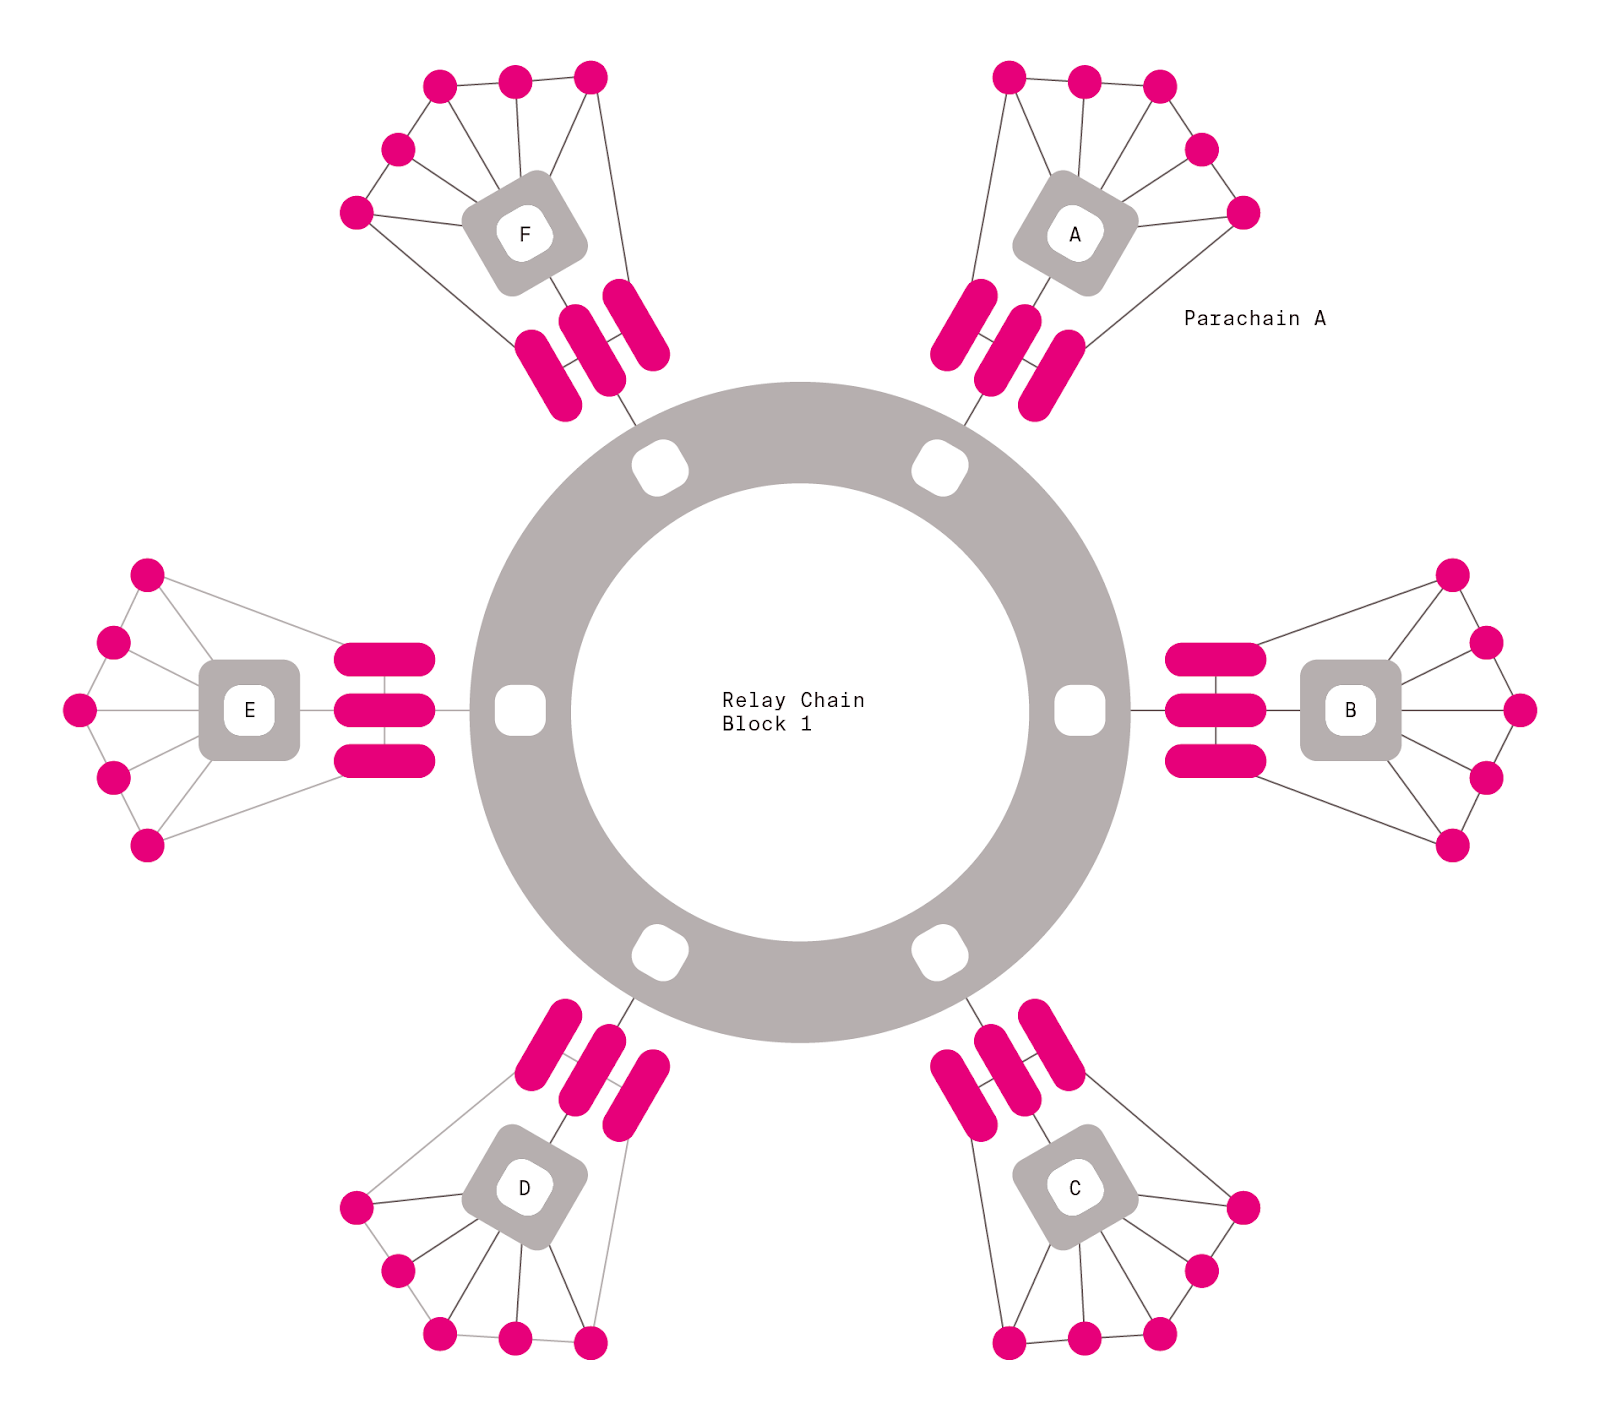
\includegraphics[width=0.7\linewidth]{polkadot_architecture.png}
  \caption{Polkadot's Architecture}
  \label{fig:polkadot_arch}
\end{figure}

Polkadot provides the bedrock relay-chain upon which a large number of validatable, globally-coherent dynamic data-structures may be hosted side-by-side.~\cite{wood2016polkadot} What has just been described are the parachains that are not obligated to be blockchains, they just must respect all the polkadot protocol.

In the Figure \ref{fig:polkadot_arch} you can see in the middle the relay chain that connects multiple parachains.

\section{Polkadot's protocol}

Briefly the Polkadot system consists of a single open collaborative decentralised network (relay chain), that interacts with many other external chains (para chains)~\cite{burdges2020overview}. For the relay chain the internals of the parachians are not relevant, parachains need only to adhere to a specific interface. The relay chain then ensure that the parachain is trustable as a whole, not single nodes.

The ecosystem expect multiple actors to make the protocol to work, the main are:
\begin{description}[font=$\bullet$ \scshape\bfseries]
  \item[Validator] Performs the bulk of the security work
  \item[Nonimator] Stakeholder who backs and selects validator candidates
  \item[Collator] Collects and submits parachain data to the relay chain
\end{description}

The protocol is composed by multiple phases and it defines the communication between parties, the main processes are:~\cite{burdges2020overview}

\begin{enumerate}
  \item The parachain's collators:
        \begin{itemize}
                \item Run full relay chain node to keep up the latest state
                \item Build new block on top of the latest state and submit blocks to the parachain's validator
        \end{itemize}
  \item The relay chain's validators:
    \begin{itemize}
      \item The ones associated to parachians produce the new relay chain block candidate
      \item Follow a sub-protocol to ensure data sharding, data are mainly parachain blocks and sharding is the process of making the validators collectively and robustly responsible for the availability of these blocks using erasure coding
      \item Submit votes to resolve forks and have a single head
      \item Manage messages between parachians
    \end{itemize}
\end{enumerate}

\subsection{State Transition Function}

The protocol demonstrate how the main goal is to verify what's happened on parachains, described by the parachain logic. One of the few required thing to a parachain is indeed a State Transition Function, this describe the parachain logic and produce the transition between two states. Like any transaction-based transition system, Polkadot state changes via an executing ordered set of instructions, known as extrinsics.~\cite{burdges2020overview}

The STF is also present in every validator node because it describe the relay chain logic. Generally STFs in polkadot are Wasm blob, currently all STFs are written in Wasm, for a parachain would be possible to use different PAB to create the STF but with complex solutions to respect what will be described later.

Every parachain or relay chain node can be divided into two parts: the STF (or Runtime) and the Client. The latter one implements everything else required to make the protocol work, from storage management to transaction gossiping.

Generally, the runtime is compiled into Wasm and stored as part of the state, this allows making fork-less upgrades because the code transition happens under consensus in the STF.

\section{Wasm in Polkadot}

Substrate is a framework to build blockchains, it is separate from Polkadot, and with it you're able to build so-called Solo Chains, a blockchain able to run on its own that does not care about the polkadot protocols.

Substrate is the main, and only for now, framework used to build blockchains in the Polkadot ecosystem, even the relay chain is built with substrate. What does substrate is abstracting all the complexity of writing client and runtime code, you have already almost everything done at client level and you have the freedom of developing whatever you want in the runtime, the state transition function of the blockchain you are building.

Substrate compiles the runtime to Wasm and the client has an embedder, wasmtime, able to run the STF. As long as the chain is a Solo Chain substrate manages everything, it compiles the runtime in wasm and implements all the custom logic to make the client and the runtime communicate through the embedder wasmtime.

The problems occur when you want to be part of the polkadot ecosystem, where there is pooled security, and the logic not only must be executed by the nodes that compose the parachain but also by the validators of the relay chain. This is made possible following a protocol made by multiple phases that are built on top of two building blocks: the Parachain Validation Function (PVF) and the Proof of Validity (PoV).~\cite{parachain-protocol}

\subsection{PVF}

Using Substrate you end up with a Substrate-Runtime, it is only a wasm blob that implements the State Transition Function of your blockchain but to be a parachain you need to provide to the relay chain something that differs a bit from the Substrate-Runtime.

The protocol requires a Parachain Validation Function that is composed of the Substrate-Runtime and another function called 'validate\_block' and the reason why this function is required is related to a constraint of the relay chain: polkadot does not know anything about the previous state of the parachain.

Everything needed by the Runtime is not present in the validators node but is provided in the block proposed by the collators, that's called: PoV, the structure of the PoV will be explained later, important to know that every information needed in the execution of the PVF is indeed in the PoV.

The 'validate\_block' function is the glue between the parachain-runtime and the PoV, it accepts the PoV and reconstructs the previous state, applies all the extrinsics using the parachain-runtime and then checks that the new state is consistent with the one proposed by the collators.

Both relay chain and parachain implement the same HostFunctions for the runtime, this means that the STF of the parachain would access the storage through the same functions in the relay chain and in the parachain but what is known by the nodes is different.

As was just said the relay chain does not know the previous state of the parachain but the information resides in the PoV. The function 'validate\_block' override the host functions to let the STF access the reconstructed internal state,present in the PoV, instead of going into the relay chain client.

\begin{figure}[h]
  \centering
  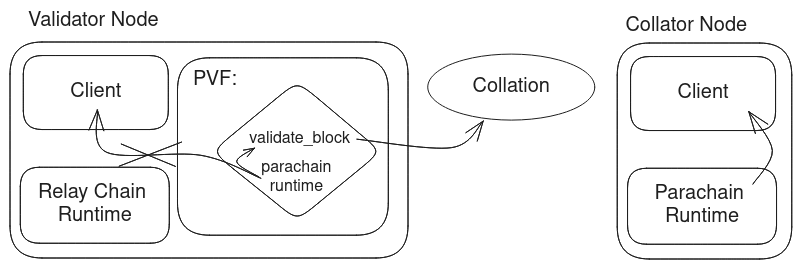
\includegraphics[width=0.8\linewidth]{validate_block_expl.png}
  \caption{PVF and Collation}
  \label{fig:pvf_pov}
\end{figure}

Collation is the term used to represent the outcome produced by the collators that will be used by validators, it is the same as PoV.

%maybe this is redundant

From the \ref{fig:pvf_pov} you can see how the parachain-runtime interacts in the same way with the embedder but it is different in the Collator or the Validator, in the first case the embedder is the client itself that knows the previous state instead in the Validator the embedder in the client is tweaked a bit so that the previous state is taken from the PoV and not from the Validator.

This encapsulation with a substitution of the host functions makes  validator able to execute different STFs without knowing anything about the parachain that is validating.

\subsection{PoV}

The Proof of Validity is made by all the things needed by Runtime Validation, it is mainly composed by:~\cite{cumulus-docs}

\begin{itemize}
  \item Header of the new block
  \item Transactions included in the block
  \item Witness Data
  \item Outgoing messages
\end{itemize}

The witness data is what makes possible the state transition validation without knowing the entire state of the parachain by the relay-chain.

The state in polkadot is represented by a key-value database where each key is unique and there is no assumption on it. The database itself is arranged as a Merkle-Patricia Base 16 Trie that allows to describe the entire state in a single constant state proof. Each block stored in the relay chain contains the state proof of the previous block, and the witness data are then composed by:


% TODO: explain Merkle-Patricia Base 16 Trie ?
% maybe poit to the repo: https://github.com/paritytech/trie

\begin{itemize}
  \item Data used in the state transition by the collator
  \item Alongside their inclusion proof in the previous state
\end{itemize}

Instead, the Outgoing messages are everything that needs to be delivered to other parachains, the underneath protocol is XCMP following the XCM format which enables the parachain communication between parachains or with the relay chain.

\subsection{SmartContracts}

SmartContracts are arbitrary codes that can be uploaded on-chain and executed in the State Transition Function. Even though the STF is arbitrary code that can be updated the convenience of SmartContracts is the easiness of creating and uploading custom logic on-chain. To make this technology different blockchain came up with different ideas and the one used by Polkadot is to have a recursive embedder.


The Client is the embedder of the STF and the STF becomes also the embedder of the SmartContracs, this is made possible thanks to Wasmi because it can be executed in wasm itself. To make the execution of arbitrary, possibly malicious, code secure there are different solutions:

\begin{itemize}
  \item Gas / Fuel measuring
  \item Storage usage deposit
\end{itemize}

Where the first one has the aim to limit the number of operations that can be executed in the STF and the second instead is to limit the amount of used storage.

\section{The crucial Role of WASM in Polkadot}

As you may understood from the above sections, the distributed algorithms, the security assumptions, all the cryptography that makes all of this possible would be useless if nodes can't execute in a secure and deterministic manner code that implements all the just described features.

The amount of tools and projects that are using Wasm makes it very suitable for polkadot, an environment with very constrained resources: there is limited space on every block, every state transition must be computed in a limited amount of time and multiple nodes must reach the same results. Wasm has already multiple tools like space and efficiency optimizer that make it even better for polkadot.

An important tools is Binaryen~\cite{binaryen} with the wasm-opt optimization phases, largely used in polkadot, that loads WebAssembly and runs Binaryen IR passes on it to make it more space and complexity efficient.

% \subsection{SPREE}
